
\part*{Ap\'{e}ndice A: Conversi\'{o}n Anal\'{o}gico-Digital.}

\newpage{}

\part*{Ap\'{e}ndice B: Conversi\'{o}n Digital-Anal\'{o}gico.}

Para convertir una se\~{n}al digital a una anal\'{o}gica despu\'{e}s
de que se ha procesado por el sistema DSP, se utiliza un conversor
D/A (o DAC, por sus siglas en ingl\'{e}s). La manera en que este proceso
se lleva a cabo es interpolando los datos de las se\~{n}ales entre
las muestras tomadas, es decir, aplicando una aproximaci\'{o}n sucesiva
al valor de dichas muestras.

La manera m\'{a}s sencilla de convertir una se\~{n}al de anal\'{o}gico
a digital, es tomando las muestras de dicha se\~{n}al desde la memoria
donde el DSP las almacena, y transformarlas en un tren de impulsos,
como se muestra en la \textbf{Figura \ref{fig:Informaci=0000F3n-digital-convertida-1}}.\textbf{
}Despu\'{e}s, este mismo tren de pulsos, se hacer pasar por un filtro
pasa bajas, con la frecuencia de corte igual a la mitad de la frecuencia
de muestreo, cumpliendo el \emph{Teorema de Nyquist}.

\begin{figure}[H]
\begin{centering}
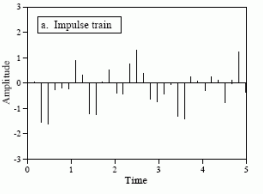
\includegraphics[scale=0.8]{img/impulse_train}
\par\end{centering}
\caption{Informaci\'{o}n digital convertida en un tren de impulsos \label{fig:Informaci=0000F3n-digital-convertida-1}.\cite{New1}}
\end{figure}

En otras palabras, la se\~{n}al original y el tren de impulsos tendr\'{a}n
espectros de frecuencia id\'{e}nticos, lo cual cumple con la \emph{frecuencia
de Nyquist} anteriormente descrita. En frecuencias m\'{a}s altas,
el tren de impulsos contiene una duplicaci\'{o}n de la se\~{n}al,
mientras que la se\~{n}al anal\'{o}gica original no contiene ninguna
informaci\'{o}n, suponiendo que el \emph{aliasing}\footnote{M\'{u}ltiples se\~{n}ales en tiempo continuo pueden producir series
de muestras id\'{e}nticas. A este fen\'{o}meno se le conoce como \emph{Aliasing}.
Cuando esto ocurre, el DAC no es cap\'{a}z de regenerar la se\~{n}al
de salida a menos que haya un filtro \emph{anti-aliasing }de por medio,
muestreando a una frecuencia mayor a la actual\cite{EECS_247}.}\textbf{\emph{ }}no ocurri\'{o}.

Mientras que este m\'{e}todo es matem\'{a}ticamente correcto, es dificil
generar esos trenes de pulsos tan estrechos entre si, utilizando componentes
electr\'{o}nicos. Para poder manejar esta dificultad, la mayor\'{\i}a
de los ADC operan manteniendo el \'{u}ltimo valor de entrada hasta
que se recibe otra muestra proveniente del DSP. A esto se le conoce
como \emph{retenci\'{o}n de \'{o}rden cero}, el equivalente del proceso
de \emph{muestra y retenci\'{o}n}\textbf{ }del DAC. La \emph{retenci\'{o}n
de orden cero }produce una se\~{n}al con apariencia de de escalera,
como se muestra en la \textbf{Figura} \ref{fig:Representaci=0000F3n-gr=0000E1fica-de-1}\footnote{Informaci\'{o}n sacada de \cite{chapter_3}.}. 

\begin{figure}[H]
\centering{}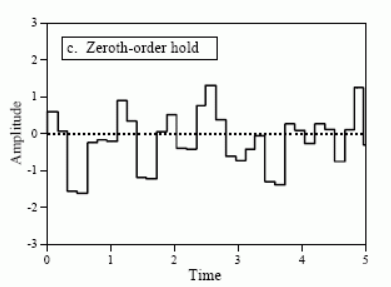
\includegraphics[scale=0.6]{img/staircase}\caption{Representaci\'{o}n gr\'{a}fica de una se\~{n}al producida por el efecto
de \emph{retenci\'{o}n de orden cero}\textbf{\emph{ }}en el proceso
de transformaci\'{o}n A/D \cite{chapter_3}\label{fig:Representaci=0000F3n-gr=0000E1fica-de-1}.}
\end{figure}

Hay diferentes formas de implementar estas conversiones D/A utilizando
componentes electr\'{o}nicos discretos y circuitos integrados, por
ejemplo\footnote{Para obtener m\'{a}s informaci\'{o}n sobre este tema, se puede referir
a \cite{binary_dacs_analogdev}, de donde se extrajo informaci\'{o}n
de esta secci\'{o}n.}
\begin{itemize}
\item \textbf{Ponderaci\'{o}n binaria: }Este DAC basado en resistores en
modo voltaje es usualmente la implementaci\'{o}n m\'{a}s simple utilizada
como referencia en los libros de texto (v\'{e}ase \textbf{Figura \ref{fig:Estructura-de-un-1}}).
No es inherentemente monol\'{\i}tico y es muy dificil de fabricar
de forma efic\'{a}z en grandes masas. Adem\'{a}s, la salida del DAC
utilizando el m\'{e}todo de ponderaci\'{o}n de voltaje binaria, cambia
con el c\'{o}digo de entrada. 
\begin{figure}[H]
\begin{centering}
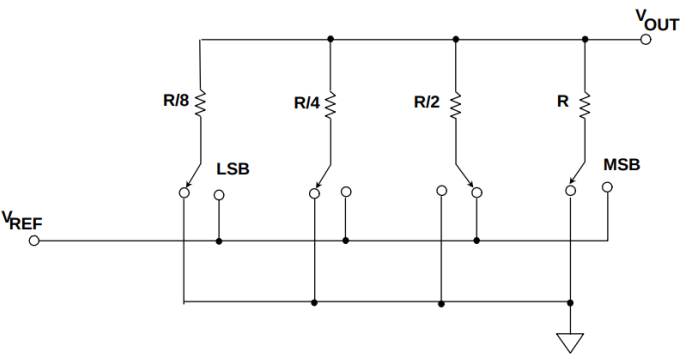
\includegraphics[scale=0.4]{img/binary_res}
\par\end{centering}
\caption{\label{fig:Estructura-de-un-1}Estructura de un DAC resistivo de ponderaci\'{o}n
binaria. Imagen adaptada de: \cite{ad_resistive_one}}
\end{figure}
\item \textbf{Ponderaci\'{o}n binaria capacitiva en aproximaci\'{o}n sucesiva:
}El uso de una redistribuci\'{o}n de carga capacitiva ofrece la ventaja
de comportarse como un circuito de muestreo y retenci\'{o}n (SHA,
por sus siglas en ingl\'{e}s), por lo cual, ning\'{u}n circuito SHA
externo o incluso, alguna construcci\'{o}n monol\'{\i}tica SHA dentro
del circuito integrado, es requerido al utilizar esta estructura (v\'{e}ase
\textbf{Figura} \ref{fig:capacitivo_ponderacion_binaria-1}). 
\begin{figure}[H]
\begin{centering}
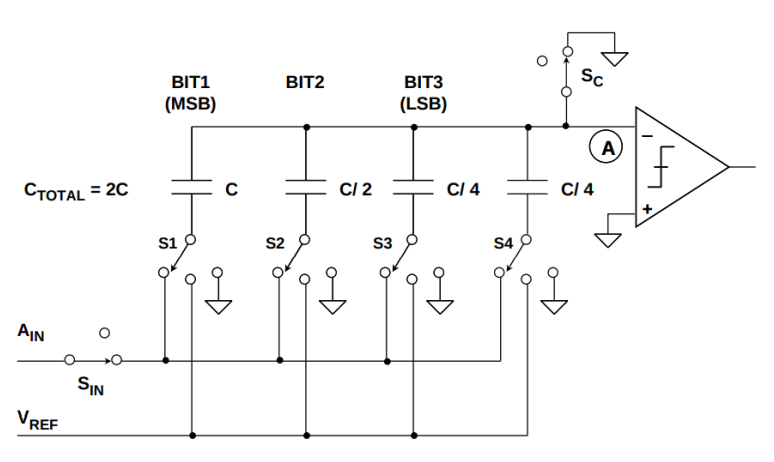
\includegraphics[scale=0.4]{img/capacitive_dac}
\par\end{centering}
\caption{\label{fig:capacitivo_ponderacion_binaria-1}Estructura de un DAC
capacitivo de ponderaci\'{o}n binaria.}
\end{figure}
\item \textbf{R-2R: }Una de las estructuras m\'{a}s comunes de DACs es la
muy conocida escalera R-2R, la cual consiste en una red de resistores
de s\'{o}lo dos diferentes valores, en una proporci\'{o}n de 2:1.
Un DAC de N bits requiere 2N resistores. El voltaje de salida se mantiene
siempre con la misma impedancia, (v\'{e}ase \textbf{Figura \ref{fig:DAC-R-2R-red-1}}).
\begin{figure}[H]
\begin{centering}
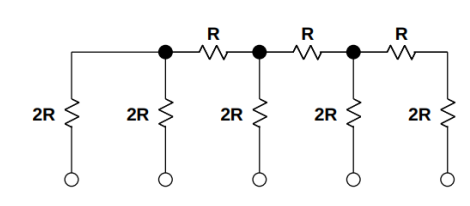
\includegraphics[scale=0.5]{img/r2r}
\par\end{centering}
\caption{\label{fig:DAC-R-2R-red-1}DAC R-2R red en escalera.}
\end{figure}
\end{itemize}
El voltaje salida de un DAC ideal se muestra en la \textbf{Figura
\ref{fig:Modelo-en-NGSpice-1}. }Para observar el c\'{o}digo Spice,
refierase al \textbf{Ap\'{e}ndice B \cite{spice_model}.}

\begin{figure}[H]
\begin{centering}
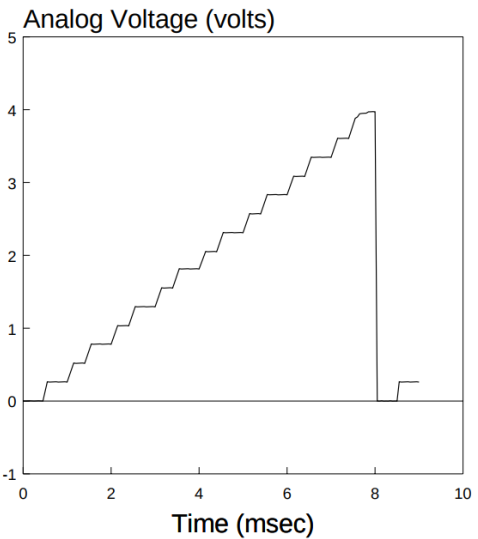
\includegraphics[scale=0.4]{img/ideal_dac}
\par\end{centering}
\caption{\label{fig:Modelo-en-NGSpice-1}Modelo en NGSpice de un DAC ideal
de 4 bits.}
\end{figure}

\newpage{}

\part*{Ap\'{e}ndice C: C\'{o}digo en Spice del DAC con respuesta ideal de
4 bits.}

\lstinputlisting[basewidth={0.5em},basicstyle={\ttfamily\small},breaklines=true,columns=flexible,keepspaces=true,language=Simula,morekeywords={WITH},tabsize=4]{src/ideal_dac.txt}

\newpage{}

\part*{Ap\'{e}ndice D: Script en Matlab de la Convoluci\'{o}n de dos vectores
de forma interactiva.}

\lstinputlisting[basewidth={0.5em},basicstyle={\ttfamily\small},breaklines=true,columns=flexible,keepspaces=true,language=Matlab,morekeywords={WITH},tabsize=4]{src/convolve_example.m}
